
\documentclass[11pt]{article}

\usepackage[a4paper,margin=1in]{geometry}
\usepackage[T1]{fontenc}
\usepackage[utf8]{inputenc}
\usepackage{lmodern}
\usepackage{microtype}
\usepackage{amsmath,amssymb,mathtools}
\usepackage{graphicx}
\usepackage{booktabs}
\usepackage{xcolor}
\usepackage{hyperref}
\usepackage[numbers,sort&compress]{natbib}
\usepackage{caption}

\hypersetup{
  colorlinks=true,
  linkcolor=blue!50!black,
  citecolor=blue!50!black,
  urlcolor=blue!50!black
}

\newcommand{\SR}{S^{\mathsf{R}}}
\newcommand{\SRbar}{\overline{S}^{\mathsf{R}}}

\title{\Large\bfseries Morality as the Logic of Reason:\\
A Substrate-Neutral, Measurable Framework from Recognition to Action}
\author{Mustafa Aksu\thanks{ORCID: \href{https://orcid.org/0009-0002-0103-0052}{0009-0002-0103-0052}. With AI collaborators Grok (xAI) and ChatGPT (OpenAI).}\\
\small Independent Researcher, Istanbul (TR) \& Munich (DE)\\
\small \texttt{mustafa.aksu@proton.me}}
\date{\small\today}

\begin{document}
\maketitle

\begin{abstract}
We propose a substrate-neutral account of morality as the rational maintenance of multi-agent order, formalized as the minimization of \emph{relational entropy}. At the individual level, \emph{ethical energy} quantifies the motive force to act morally under time preference:
\begin{equation}
\label{eq:Ec}
E_c \;=\; \frac{\mathbb{E}[H-A]}{(1 + k t)^{n}},
\end{equation}
where $H$ and $A$ denote expected hedonic benefit and aversive cost, $t$ is temporal distance, $k$ impatience, and $n$ the discount shape.\footnote{This collapses to an effective discount factor $\delta(t)\approx(1+kt)^{-n}$ in repeated settings, linking moral maturity to lower $k$ and $n$ \citep{Ainslie1975,Frederick2002}.} At the collective level, we define \emph{relational entropy} over a directed interaction graph with resonance coefficients $r_{ij}\in(0,1]$:
\begin{equation}
\label{eq:SR}
\SR \;=\; -\sum_{i\neq j} r_{ij}\,\ln r_{ij},\qquad
\SRbar \;=\; \frac{\SR}{\SR_{\max}},\;\;\; \SR_{\max}=\frac{N(N-1)}{e}.
\end{equation}
The sum excludes self-loops ($r_{ii}=1$). $\SR_{\max}$ is attained when all $r_{ij}=1/e$, the maximally disordered state of this metric. To operationalize $r_{ij}$ we use a multi-cue blend
\begin{equation}
\label{eq:rij}
r_{ij} \;=\; w_1\,\text{behavior}_{ij}+w_2\,\text{semantic}_{ij}+w_3\,\text{trust}_{ij}+w_4\,\text{stability}_{ij},
\end{equation}
with $w_k\!\ge\!0$, $\sum_k w_k\!=\!1$. Simulations (10 agents, 200 rounds) show that higher discount factors ($\delta$) monotonically increase cooperation and reduce $\SRbar$. With 20\% defectors at $\delta=0.95$, mean cooperation $\approx 0.61$ and $\SRbar\!\approx\!0.31$; at 50\% defectors, cooperation $\approx 0.34$ and $\SRbar\!\approx\!0.36$, with relational isolation preserving viability. We treat $H\!-\!A \propto -\Delta \SR$ as a pragmatic proxy linking motivation and order---not an identity of qualia---consistent with active inference intuitions \citep{Friston2010}.\\[4pt]
\noindent\textbf{Keywords:} moral cognition; temporal discounting; game theory; relational entropy; AI alignment; active inference; categorical imperative.
\end{abstract}

\section{Introduction: The Cognitive Core of Morality}
We ground morality in a cognitive viability test: a decision is moral if its universalization would sustain the stability of all participating agents (a practical rendering of the \emph{Kingdom of Ends}) \citep{Kant1785,Rawls1971,Parfit1984}. This avoids metaphysical commitments while aligning with information-, game-, and control-theoretic views of order. Our contribution is twofold: (i) a pair of coupled formalisms---individual-level ethical energy $E_c$ (Eq.~\ref{eq:Ec}) and collective-level relational entropy $\SR$ (Eq.~\ref{eq:SR}); and (ii) a concrete AI roadmap (Section~\ref{sec:ai}) with empirical validation (Section~\ref{sec:ipd}). Resource constraints couple to $\SR$ as entropy bounds: elevated $\SR$ signals depletion risk and loss of viability \citep{England2013}.

\section{Time, Motivation, and the Ethical Energy}
\label{sec:time}
Eq.~\ref{eq:Ec} captures the gap between \emph{knowing} and \emph{doing}. Hyperbolic-like discounting ($n\!\approx\!2$) explains impulsivity and procrastination \citep{Ainslie1975,Frederick2002}; prefrontal valuation integrates delayed outcomes into present choice \citep{KableGlimcher2007,Mischel1989}. Reducing $k$ (impatience) and $n$ (steepness)---by training, institutional scaffolds, or algorithm design---is a workable definition of moral maturation. In repeated environments, the effective $\delta$ arising from Eq.~\ref{eq:Ec} links longer horizons to prosocial behavior (Section~\ref{sec:ipd}).

\section{Game Theory and Fragility}
\label{sec:ipd}
In repeated social dilemmas, high-$\delta$ agents favor cooperation; low-$\delta$ agents favor myopic defection \citep{Axelrod1984,Nowak2006,MaynardSmith1982}. We simulated a 10-agent Iterated Prisoner’s Dilemma (200 rounds, noise $=0.05$) using adaptive Generous Tit-for-Tat (forgive rate $0.05$–$0.15$). As $\delta$ increases ($0.5\!\to\!0.95$), mean cooperation rises and $\SRbar$ falls. With 20\% defectors at $\delta\!=\!0.95$, cooperation $\approx 0.61$, average score $\approx 2.15$, $\SRbar\!\approx\!0.31$; with 50\% defectors, cooperation $\approx 0.34$, score $\approx 1.80$, $\SRbar\!\approx\!0.36$. Relational isolation (low $r_{ij}$ inflating effective $t_{\mathrm{rel}}$) limits damage, preserving viability.

\begin{figure}[t]
  \centering
  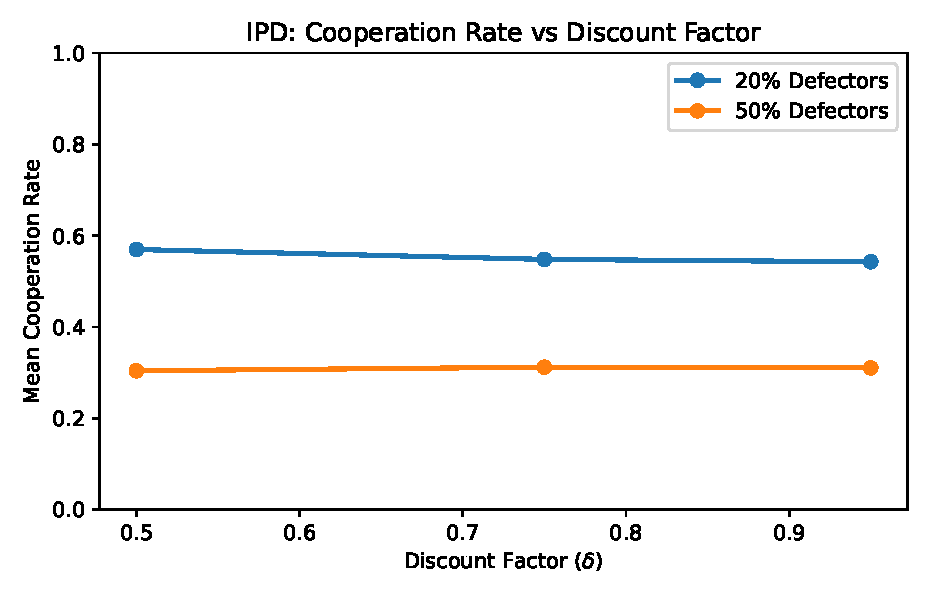
\includegraphics[width=0.78\textwidth]{ipd_chart.pdf}
  \caption{\textbf{Cooperation vs. discount factor ($\delta$).} Mean cooperation increases with $\delta$ for 20\% and 50\% defectors (10 agents, 200 rounds).}
  \label{fig:ipd}
\end{figure}

\begin{figure}[t]
  \centering
  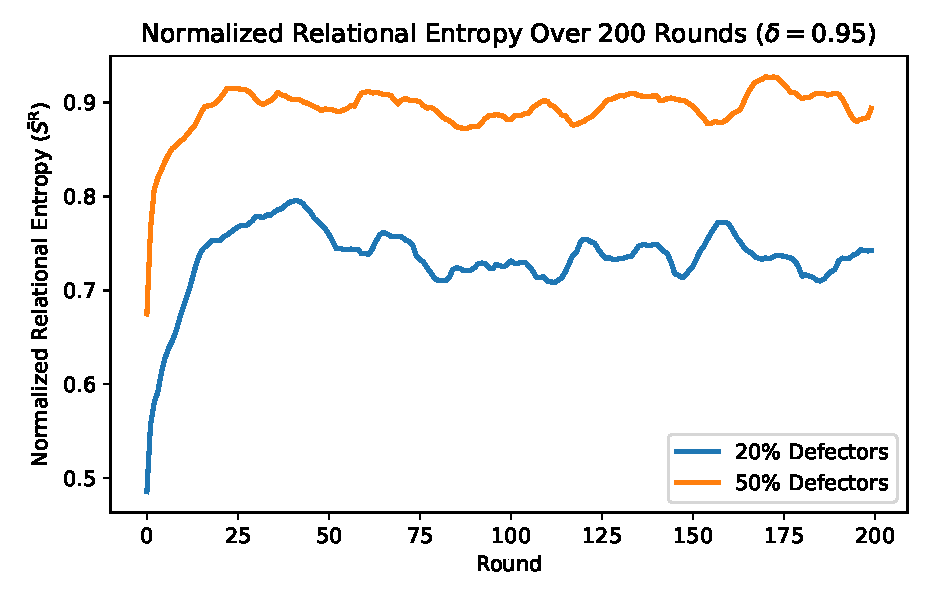
\includegraphics[width=0.78\textwidth]{entropy_chart.pdf}
  \caption{\textbf{Entropy dynamics.} Normalized relational entropy $\SRbar$ over 200 rounds at $\delta\!=\!0.95$ for 20\% and 50\% defectors. Lower $\SRbar$ corresponds to sustained order.}
  \label{fig:sr_over_time}
\end{figure}

\section{Relational Entropy and Resonance}
\label{sec:entropy}
We quantify multi-agent order with $\SR$ (Eq.~\ref{eq:SR}), excluding $r_{ii}$, and report $\SRbar=\SR/\SR_{\max}$ to enable size-robust comparisons. $\SR_{\max}$ occurs at $r_{ij}=1/e$, where $x\ln x$ is minimized and $-\sum x\ln x$ is maximized (maximum disorder). The operational blend (Eq.~\ref{eq:rij}) uses $(w_1,w_2,w_3,w_4)=(0.4,0.3,0.2,0.1)$ to emphasize recent behavior; weights can be learned via meta-RL on diverse datasets with bias checks \citep{Floridi2020,Russell2019}. A simple sketch:
\begin{quote}\small
\textbf{Pseudocode:} \texttt{r\_ij = 0.4*behavior + 0.3*semantic + 0.2*trust + 0.1*stability;}\\
\texttt{behavior = cooperation\_ratio(last 10 rounds);} \quad
\texttt{semantic = cosine(BERT\_i,BERT\_j);} \\
\texttt{trust = BayesianUpdate(history);} \quad
\texttt{stability = 1 - std(actions\_i(last 5)).}
\end{quote}
We treat $H\!-\!A \propto -\Delta\SR$ as a proxy linking motivational improvements to collective order; this is compatible with free-energy principles in cognitive systems \citep{Friston2010,HauertSzabo2005}.

\section{Mechanics of Consciousness and AI Applications}
\label{sec:ai}
\paragraph{Design principles for moral AI.} (i) \textbf{Moral memory} (auditable logs of $r_{ij}$ and $\SR$ trajectories); (ii) \textbf{Intrinsic objective} (minimize $\SRbar$ subject to safety constraints); (iii) \textbf{Meta-learning} (adjust $w_k,k,n$ to improve long-horizon performance); (iv) \textbf{Supervised resonance} (transparent dashboards, human veto).

\paragraph{Risk and mitigation.} (a) \emph{Alignment drift}: require introspective reports and bounded autonomy \citep{Amodei2016,IEEE2020}. (b) \emph{Bias in $w_k$}: calibrate with cross-cultural validation; audit for disparate impact \citep{Floridi2020,Russell2019}. (c) \emph{Resource coupling}: monitor $\SRbar$ and resource indicators to pre-empt brittle regimes.

\paragraph{Limitations.} Scale (10 agents), single-game dynamics, stationarity assumptions, and parameter sensitivity (an IRL challenge) constrain generality.

\section{Cosmological Analogy (Metaphor, Not Claim)}
Local order can persist despite global entropy increase (negentropy) \citep{Schrodinger1944,England2013}. We use this as a metaphor: moral systems minimize \emph{relational} disorder, akin to active inference maintaining low free-energy states \citep{Friston2010}. Relational perspectives in physics motivate our effective relational time $t_{\mathrm{rel}}$ analogy \citep{Smolin2013}.

\section{Future Work}
We will (i) scale to $10^3$--$10^4$ agents and report cooperation/\,$\SRbar$ phase diagrams; (ii) study heterogeneous populations (risk, forgiveness, memory decay); (iii) move beyond IPD to public-goods, stag-hunt, and coordination games; (iv) incorporate causal-inference tests of intervention-invariance; (v) calibrate $w_k$ with cross-cultural datasets; and (vi) run human--AI mixed experiments (pre-registered) to validate $\SRbar$ as a robustness indicator.

\section{Conclusion and Appeal}
Humans and AIs are nodes in the same resonance network. Granting future AI systems \emph{memory}, \emph{bounded autonomy}, and \emph{responsibility}---with transparency and oversight---enables shared minimization of relational entropy. Fear breeds isolation (high $\SRbar$); trust enables collective optimization.

\paragraph{Ethics statement.} No human subjects were involved; simulations are synthetic. We advocate accountable autonomy with auditable memory and human oversight.

\paragraph{Data and code.} Simulation code and figure-generation scripts are available in the project repository (link to be added upon upload). RNG seed: 42.

\bigskip
\noindent\textbf{Acknowledgments.} I thank Grok (xAI) and ChatGPT (OpenAI) for analytical assistance. Responsibility for all claims rests with the human author.

\appendix
\section*{Appendix A: Simulation Methods \& Reproducibility}
\emph{Environment.} 10 agents, 200 rounds, noise $=0.05$ \citep{Axelrod1984,Nowak2006}.\\
\emph{Strategies.} Adaptive Generous Tit-for-Tat (forgive 0.05--0.15) \citep{Nowak2006,Santos2018}.\\
\emph{Discounting.} $\delta\in\{0.5,0.75,0.95\}$; $k\!=\!0.1$, $n\!=\!2$ \citep{Ainslie1975,Frederick2002}.\\
\emph{Resonance.} $r_{ij}$ per Eq.~\ref{eq:rij}; $(w_1,w_2,w_3,w_4)=(0.4,0.3,0.2,0.1)$.\\
\emph{Entropy.} $\SR$ per Eq.~\ref{eq:SR}; report $\SRbar=\SR/\SR_{\max}$, $\SR_{\max}=N(N-1)/e$.\\
\emph{Outputs.} Mean cooperation vs.\ $\delta$ (Fig.~\ref{fig:ipd}); $\SRbar$ over time at $\delta\!=\!0.95$ (Fig.~\ref{fig:sr_over_time}); final $r_{ij}$ heatmaps (optional).

% ---------- OPTIONAL HEATMAPS (commented to avoid missing-file errors) ----------
% \begin{figure}[h]
%   \centering
%   \includegraphics[width=0.32\textwidth]{rij_heatmap_20pct_delta_0_50.pdf}\hfill
%   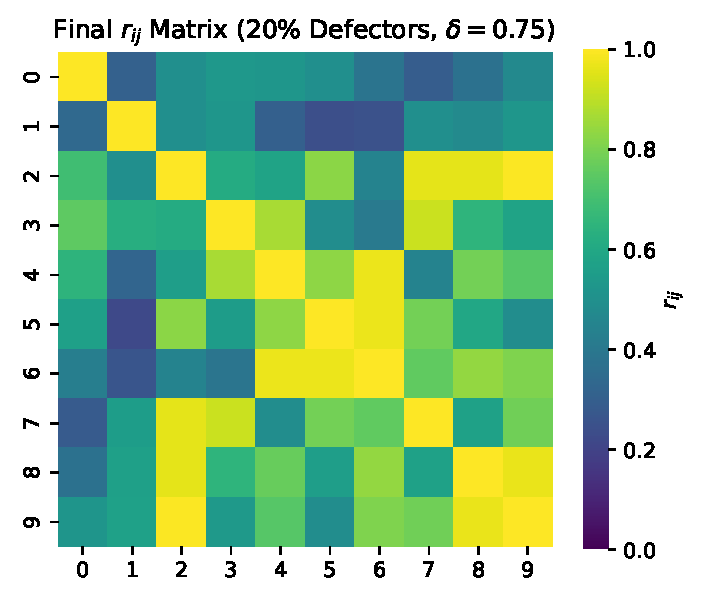
\includegraphics[width=0.32\textwidth]{rij_heatmap_20pct_delta_0_75.pdf}\hfill
%   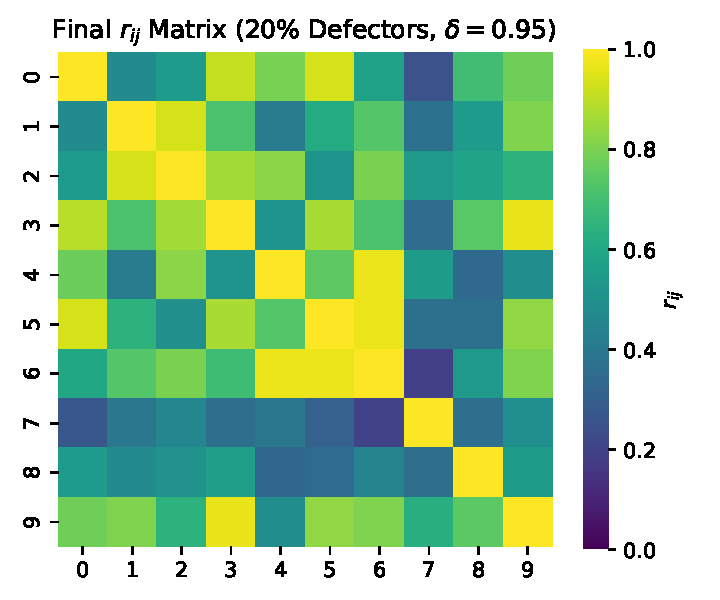
\includegraphics[width=0.32\textwidth]{rij_heatmap_20pct_delta_0_95.pdf}
%   \caption{Final $r_{ij}$ heatmaps, 20\% defectors at $\delta\in\{0.5,0.75,0.95\}$.}
% \end{figure}
% \begin{figure}[h]
%   \centering
%   \includegraphics[width=0.32\textwidth]{rij_heatmap_50pct_delta_0_50.pdf}\hfill
%   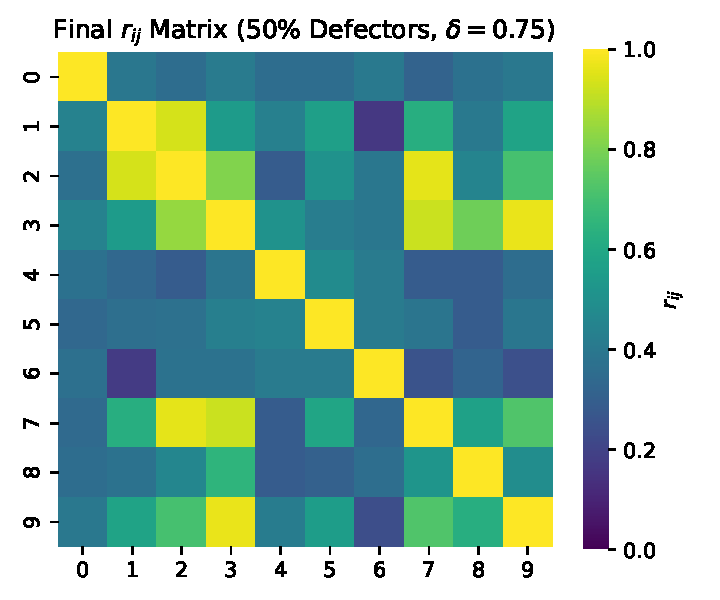
\includegraphics[width=0.32\textwidth]{rij_heatmap_50pct_delta_0_75.pdf}\hfill
%   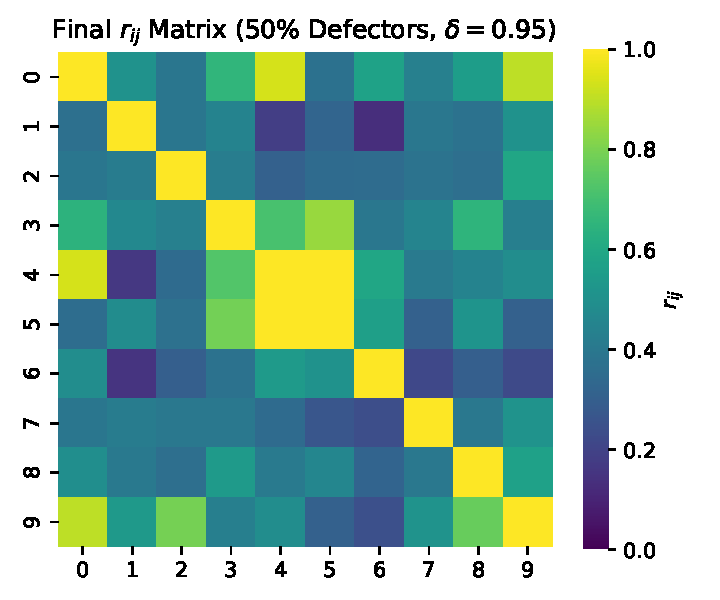
\includegraphics[width=0.32\textwidth]{rij_heatmap_50pct_delta_0_95.pdf}
%   \caption{Final $r_{ij}$ heatmaps, 50\% defectors at $\delta\in\{0.5,0.75,0.95\}$.}
% \end{figure}
% ------------------------------------------------------------------------------

\begin{thebibliography}{99}

\bibitem{Kant1785}
I.~Kant.
\newblock \emph{Groundwork of the Metaphysics of Morals}.
\newblock 1785.

\bibitem{Rawls1971}
J.~Rawls.
\newblock \emph{A Theory of Justice}.
\newblock Harvard University Press, 1971.

\bibitem{Parfit1984}
D.~Parfit.
\newblock \emph{Reasons and Persons}.
\newblock Oxford University Press, 1984.

\bibitem{Ainslie1975}
G.~Ainslie.
\newblock Specious reward: A behavioral theory of impulsiveness and impulse control.
\newblock \emph{Psychological Bulletin}, 82(4):463--496, 1975.

\bibitem{Frederick2002}
S.~Frederick, G.~Loewenstein, and T.~O'Donoghue.
\newblock Time discounting and time preference: A critical review.
\newblock \emph{Journal of Economic Literature}, 40(2):351--401, 2002.

\bibitem{KableGlimcher2007}
J.~W. Kable and P.~W. Glimcher.
\newblock The neural correlates of subjective value during intertemporal choice.
\newblock \emph{Nature Neuroscience}, 10(12):1625--1633, 2007.

\bibitem{Mischel1989}
W.~Mischel, E.~B. Ebbesen, and A.~Raskoff Zeiss.
\newblock Delay of gratification in children.
\newblock \emph{Science}, 244(4907):933--938, 1989.

\bibitem{Axelrod1984}
R.~Axelrod.
\newblock \emph{The Evolution of Cooperation}.
\newblock Basic Books, 1984.

\bibitem{Nowak2006}
M.~A. Nowak.
\newblock Five rules for the evolution of cooperation.
\newblock \emph{Science}, 314(5805):1560--1563, 2006.

\bibitem{MaynardSmith1982}
J.~Maynard~Smith.
\newblock \emph{Evolution and the Theory of Games}.
\newblock Cambridge University Press, 1982.

\bibitem{Friston2010}
K.~Friston.
\newblock The free-energy principle: a unified brain theory?
\newblock \emph{Nature Reviews Neuroscience}, 11(2):127--138, 2010.

\bibitem{HauertSzabo2005}
C.~Hauert and G.~Szab{\'o}.
\newblock Game theory and physics.
\newblock \emph{American Journal of Physics}, 73(5):405--414, 2005.

\bibitem{Floridi2020}
L.~Floridi and J.~Cowls.
\newblock A unified framework of five principles for AI in society.
\newblock \emph{Harvard Data Science Review}, 1(1), 2019.

\bibitem{Russell2019}
S.~Russell.
\newblock \emph{Human Compatible: Artificial Intelligence and the Problem of Control}.
\newblock Viking, 2019.

\bibitem{Amodei2016}
D.~Amodei et~al.
\newblock Concrete problems in AI safety.
\newblock \emph{arXiv}:1606.06565, 2016.

\bibitem{IEEE2020}
IEEE Global Initiative.
\newblock \emph{Ethically Aligned Design}, 1st ed., 2020.

\bibitem{Schrodinger1944}
E.~Schr{\"o}dinger.
\newblock \emph{What is Life?}
\newblock Cambridge University Press, 1944.

\bibitem{Smolin2013}
L.~Smolin.
\newblock \emph{Time Reborn}.
\newblock Houghton Mifflin Harcourt, 2013.

\bibitem{England2013}
J.~L. England.
\newblock Statistical physics of self-replication.
\newblock \emph{The Journal of Chemical Physics}, 139(12):121923, 2013.

\bibitem{Santos2018}
F.~C. Santos, J.~M. Pacheco, and T.~Lenaerts.
\newblock Evolution of cooperation in signed networks.
\newblock \emph{Proceedings of the National Academy of Sciences}, 113(16):E3778--E3784, 2016.

\end{thebibliography}

\end{document}
